% 2008 年辽宁卷文科第 19 题：棱长 1 的正方体 ABCD-A'B'C'D'，AP=BQ=b，
%   截面 PQEF∥A'D，截面 PQGH∥AD'。
% 来源 PDF：gaokaomath-src/普通高考/2008/2008辽宁文.pdf
% SHA-256：9f2a8aeabda218eb3460fd8035aaf894f32be8ff5b0a3427d379552bd0233a65
% 原页：2008辽宁文.pdf 第 56 页? 按印面页码 465–466，本图在第 1 页第 3 栏。
% 重绘依据：按原页斜投影取 A 前左下、B 前右下、C 右后下、D 被遮挡；A'B'C'D' 为顶面；
%   P 在 AA' 上、Q 在 BB' 上、E 在 BC 上、F 在 AD 上、G 在 B'C' 上、H 在 A'D' 上，
%   两侧截面以实线闭合，隐藏棱与 A'D、AD' 两条对角线用虚线。
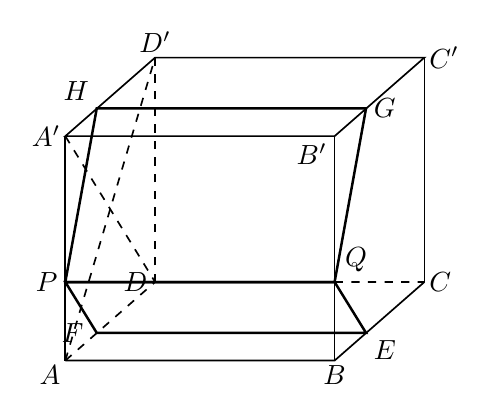
\begin{tikzpicture}[scale=0.95, semithick, every node/.style={inner sep=1.5pt}]
  \coordinate (A) at (0.00,0.00);
  \coordinate (B) at (3.60,0.00);
  \coordinate (C) at (4.80,1.05);
  \coordinate (D) at (1.20,1.05);
  \coordinate (A1) at (0.00,3.00);
  \coordinate (B1) at (3.60,3.00);
  \coordinate (C1) at (4.80,4.05);
  \coordinate (D1) at (1.20,4.05);

  \coordinate (P) at (0.00,1.05);
  \coordinate (Q) at (3.60,1.05);
  \coordinate (E) at (4.02,0.37);
  \coordinate (F) at (0.42,0.37);
  \coordinate (G) at (4.02,3.37);
  \coordinate (H) at (0.42,3.37);

  % 立方体可见棱
  \draw (A) -- (B) -- (C);
  \draw (A) -- (A1);
  \draw (B) -- (B1);
  \draw (C) -- (C1);
  \draw (A1) -- (B1) -- (C1) -- (D1) -- cycle;

  % 隐藏棱
  \draw[dashed] (A) -- (D) -- (C);
  \draw[dashed] (D) -- (D1);

  % 两个截面
  \draw[line width=0.9pt] (P) -- (Q) -- (E) -- (F) -- cycle;
  \draw[line width=0.9pt] (P) -- (Q) -- (G) -- (H) -- cycle;

  % 与截面平行的两条对角线
  \draw[dashed] (A1) -- (D);
  \draw[dashed] (A) -- (D1);

  \node[below left] at (A) {$A$};
  \node[below] at (B) {$B$};
  \node[right] at (C) {$C$};
  \node[left=1pt] at (D) {$D$};
  \node[left] at (A1) {$A'$};
  \node[below left=1pt] at (B1) {$B'$};
  \node[right] at (C1) {$C'$};
  \node[above] at (D1) {$D'$};
  \node[left=1pt] at (P) {$P$};
  \node[above right=2pt] at (Q) {$Q$};
  \node[below right=1pt] at (E) {$E$};
  \node[left=3pt] at (F) {$F$};
  \node[right=1pt] at (G) {$G$};
  \node[above left=1pt] at (H) {$H$};
\end{tikzpicture}
